\chapter{Comparative Study}~\label{ch:comparative study}

This chapter deals with a systematic evaluation of the previously investigated methods for creating 3D models. This analysis is crucial for understanding the real-world applicability and effectiveness of each method. The aim is to compare the theoretical principles with the practical results and to provide a comprehensive evaluation of the performance of each model under experimental conditions.

The chapter begins with a description of the experimental setup that was created to test these methods. This includes the specific conditions, frameworks and parameters used to ensure that the comparison is fair and the results reliable. 
The generation process of the same example prompt is then shown for each method. This section shows all the steps required to bring the result of each method into its final form in several iterations. Finally, the chapter highlights a thorough analysis of the results obtained from these experiments. This section not only presents the data, but also interprets them in the context of the theoretical background, limitations and potential applications of each method. The insights gained here are helpful for anyone who wants to understand the state of the art in 3D modeling and its practical implications in the real world.

\section{Experimental Setup}\label{Setup}

3D model generation is a demanding task, both in terms of computational power and hardware resources. Each method has unique requirements, which poses a significant challenge in creating a fair baseline for comparative analysis.

To address this, the project Threestudio \citep{threestudio2023} was utilized. This platform provides slightly adapted versions of the official methods, preserving their core functionality while making them more accessible for systems with limited hardware capabilities. Magic123 \citep{qian2023magic123}, for example, was originally tested on a V100 GPU with about 32 GB RAM, but Threestudio's version also works on a T4 GPU with about 15 GB RAM.\@. This adjustment ensures uniform testing conditions across various methods, enabling fair comparisons without the need for high-end hardware. However, this benefit comes at the cost of extended training times and inferior outputs compared to the original versions. Threestudio's specific modifications can be found in their GitHub documentation \citep{threestudio2023}.

Despite the advantages of Threestudio, hardware limitations were still a major problem. The available hardware for this thesis was a single NVIDIA GeForce RTX 2080 GPU with 8 GB of RAM\@. Therefore, Google Colab \citep{googlecolab} was used to mitigate these limitations as it provides access to free GPUs and the ability to run code efficiently.

However, this approach had its own limitations. Colab is limited to a single GPU, whereas most 3D generation methods typically benefit from training with multiple GPUs, to achieve more detailed results and faster computation times. Table 1 shows the differences in training duration for each method, highlighting the gap between personal hardware capabilities and the requirements of the original implementations. Another notable limitation of Google Colab is its unpredictability in terms of how long a notebook can be used before the runtime is reset. Opting for the premium version of Colab can mitigate this issue by providing a more stable runtime, but this comes with a subscription fee.

Threestudio provided a test Colab notebook with an initial implementation for DreamFusion. This setup was further refined and extended by myself to improve its functionality and usability. Changes included the ability to transfer the complete training folder with checkpoints, validation images, configuration details and outputs to Google Drive for easy data access and storage. In addition, this improved notebook now includes comprehensive code snippets for training, refining and exporting for each model beyond the scope of Dreamfusion. To prevent common computational errors due to varying dependencies, additional packages were integrated into the setup.

To unite all the methods used in one notebook, the official implementation of Wonder3D \citep{long2023wonder3d} is also included in the notebook, as well as Evaluate3D, a tool I developed myself for basic geometric comparisons of object files 

It is worth mentioning that the functionality of this notebook is strongly based on Threestudio's guidelines, and as the project evolves, some personal adjustments might be superseded by updates from the authors.



\section{Individual Generation Process}\label{generationProcess}

If not mentioned differently, each model was trained for 10,000 iterations using a single T4 GPU in Google Colab with the High-Ram setting enabled. It is important to note that this hardware configuration does not match the specifications used in the official implementations of these models. Consequently, the results generated in this study may not be as detailed and precise. Despite these limitations, the primary purpose here is to evaluate the basic capabilities of each model, which is possible even with comparatively modest hardware standards.

To effectively demonstrate the generation process of each method, an example prompt was used: ``a robot made of plants''. The choice of this prompt was strategic as concept of a robot is inherently versatile and does not have a rigid definition in terms of appearance or composition. Furthermore, it was assumed that a simple prompt such as ``a robot'' would lead to bland models, reflecting the results observed when applying such a prompt to a 2D diffusion model, specifically Dall-E 3 \citep{dalle3}. To mitigate this, the phrase ``made out of plants'' was added. This not only countered the potential monotony of the models, but also tested the models' ability to represent intricate detail and incorporate color, particularly the various hues associated with plants. The expectation was that this addition would enrich the output of the models and provide a more comprehensive basis for evaluating their detail rendering capabilities.

\textbf{Dreamfusion}~--~The model begins by initializing an object randomly and then refines it throughout the training process. Each prompt initiates the creation of a distinct scene, meaning that even repeated usage of the same text input generates unique objects. This phenomenon is evident in the results presented in Figure~\ref{fig:generationDreamFusion}, and Figure~\ref{fig:secondRobotDreamfusion} included in the Appendix. The entire training process typically spans approximately 1.5 hours, with each iteration consuming a consistent amount of time.

\begin{figure}[ht]
    \centering
    % Subfigure for textual description
    \begin{subfigure}[b]{0.20\textwidth}
        \centering
        \fontsize{9pt}{7pt}\selectfont\text{Iteration = 100}\vspace{3cm}
        \fontsize{9pt}{7pt}\selectfont\text{Iteration = 5000}\vspace{2.85cm}
        \fontsize{9pt}{7pt}\selectfont\text{Iteration = 10000}\vspace{1.95cm}
    \end{subfigure}
    \begin{subfigure}[b]{0.20\textwidth}
        \centering
        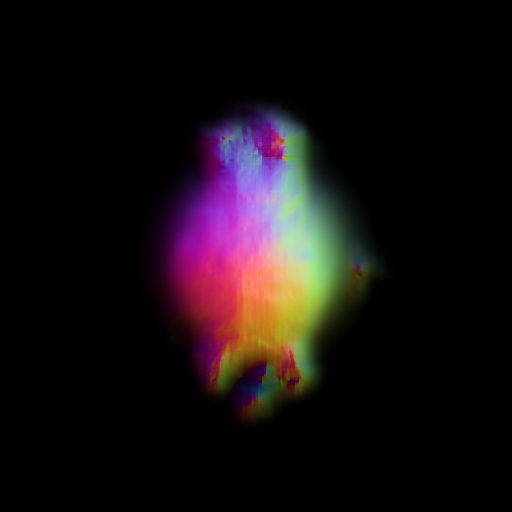
\includegraphics[width=\textwidth]{etc/a robot made out of plants/dreamfusion/dreamfusion_plantrobot_1_part2.png}
        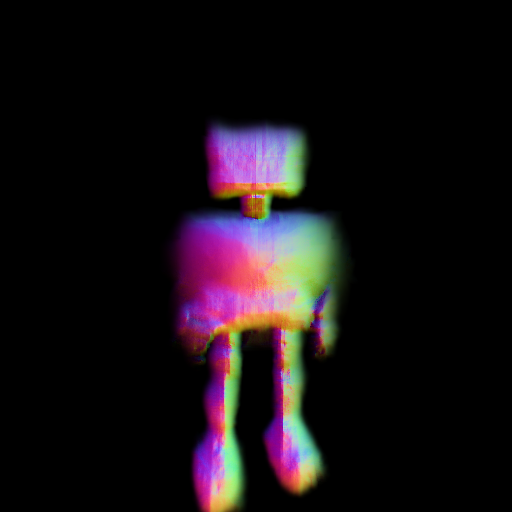
\includegraphics[width=\textwidth]{etc/a robot made out of plants/dreamfusion/dreamfusion_plantrobot_5000_part2.png}
        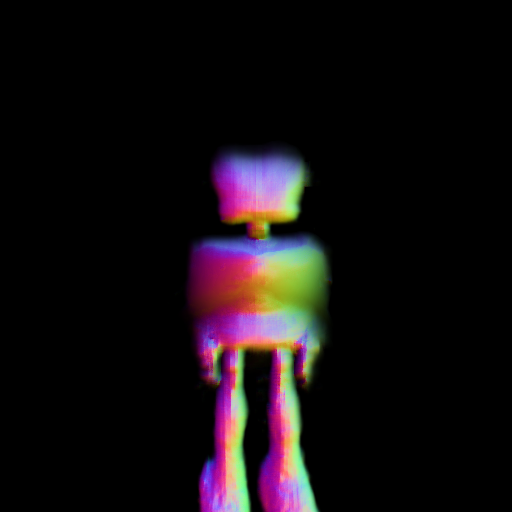
\includegraphics[width=\textwidth]{etc/a robot made out of plants/dreamfusion/dreamfusion_plantrobot_10000_part2.png}
        \caption{}
    \end{subfigure}
    \begin{subfigure}[b]{0.20\textwidth}
        \centering
        
\includegraphics[width=\textwidth]{etc/a robot made out of plants/dreamfusion/dreamfusion_plantrobot_1_part1.png}
        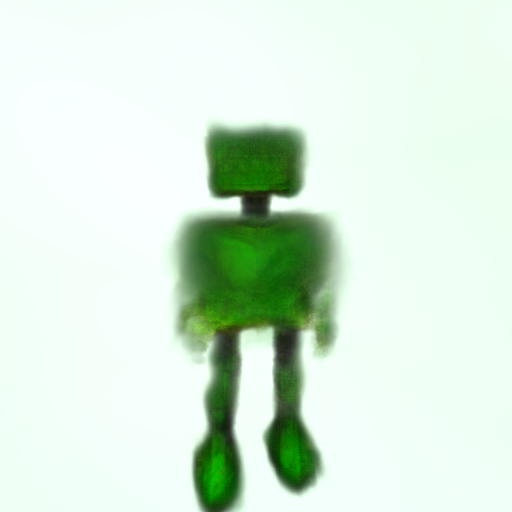
\includegraphics[width=\textwidth]{etc/a robot made out of plants/dreamfusion/dreamfusion_plantrobot_5000_part1.png}
        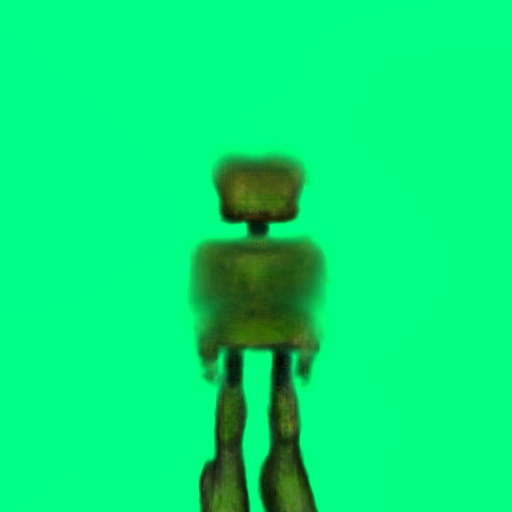
\includegraphics[width=\textwidth]{etc/a robot made out of plants/dreamfusion/dreamfusion_plantrobot_10000_part1.png}
        \caption{}
    \end{subfigure}
    % Subfigure 3
    \hspace{.5cm}
    \begin{subfigure}[b]{0.252\textwidth}
        \centering
        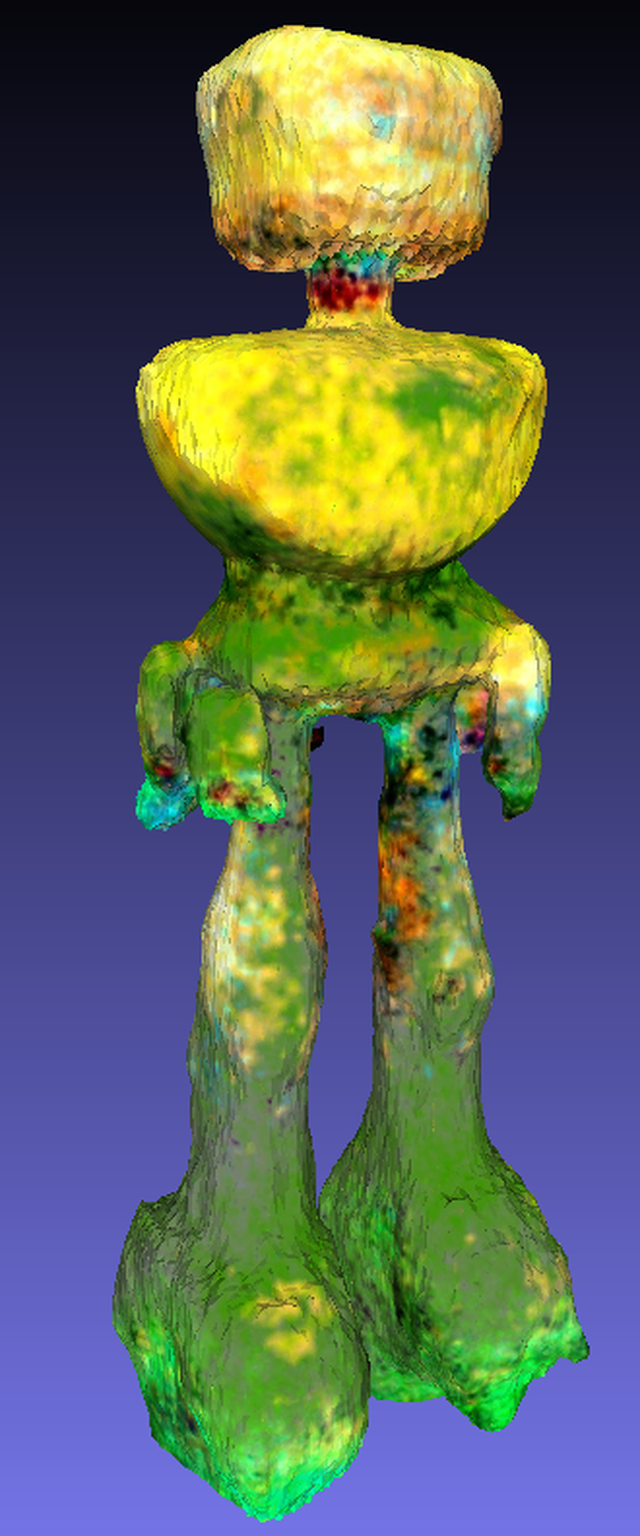
\includegraphics[width=\textwidth]{etc/a robot made out of plants/dreamfusion/dreamfusion_plantrobot_model_resized.png}
        \caption{}
    \end{subfigure}
    \caption{The generation process of Dreamfusion using the prompt ``a robot made out of plants''. Section (c) shows a snapshot of the final mesh generated.}~\label{fig:generationDreamFusion}
\end{figure}

As seen in Figure~\ref{fig:generationDreamFusion} parts (a) and (b), the object and its texture are generated simultaneously. The process starts with a small dot that gradually transforms into a more complex shape. At the 100th iteration, the original dot begins to transform into a recognizable shape, and a green hue resembling plant coloration is created. At the 5000th iteration, distinct features such as two legs, a square body and a square head become visible, all retaining the same shade of green. At the last, 10,000th iteration, the model shows a background and small arms sticking out of the robot's body.
Part c of the figure showcases the rendered mesh opened in Meshlab \citep{meshLab}, highlighting alterations made by Threestudio, such as duplicate removal and hole filling. These modifications account for the slight differences between the final mesh and the validation images produced during training. Interestingly, the final mesh lacks detailed plant-like features, one could only assume that the legs kind of resemble moss, but this remains speculation. The mesh primarily shows basic shapes, including a square head, a torso with small protruding rods that could be arms, and large legs. Remarkably, the upper half of the body in the final mesh takes on a yellowish color that differs from the green of the earlier validation images. The reason for this color change remains unclear.

\textbf{Fantasia3D}~--~There are several ways to initiate the generation of 3D models in Fantasia3D. The most straightforward method, used in this section, is to begin with just the prompt, wherein Fantasia3D defaults to using a sphere as the initial mesh, shaping the training process from this starting point. Alternatively, one can customize the sphere's initial values  \([0.5, 0.5, 0.5]\) to better represent the desired object by adjusting the parameters to correspond to \([depth, width, height]\). The final approach involves initializing the mesh with a custom~.obj file, providing a rough outline of the intended shape. An example of the latter approach can be seen in Figure~\ref{fig:generationFantasia2} in the appendix, where the generation process was started with a rough human figure.

\begin{figure}[ht]
    \centering
    % Subfigure for textual description
    \begin{subfigure}[b]{0.20\textwidth}
        \centering
        \fontsize{9pt}{7pt}\selectfont\text{Iteration = 0}\vspace{3cm}
        \fontsize{9pt}{7pt}\selectfont\text{Iteration = 5000}\vspace{2.85cm}
        \fontsize{9pt}{7pt}\selectfont\text{Iteration = 10000}\vspace{1.95cm}
    \end{subfigure}
    \begin{subfigure}[b]{0.20\textwidth}
        \centering
        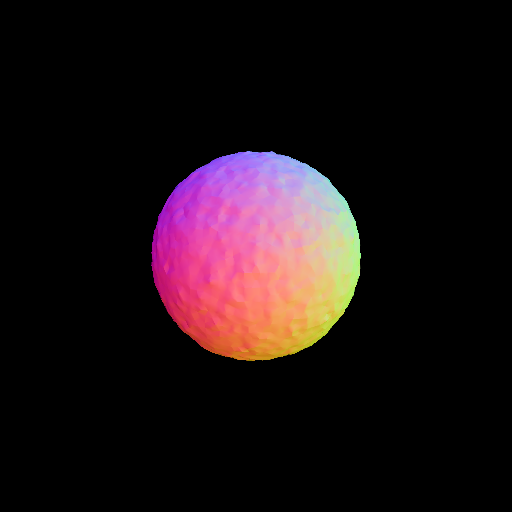
\includegraphics[width=\textwidth]{etc/a robot made out of plants/fantasia3d/fantasia_coarse_robot_0_part2.png}
        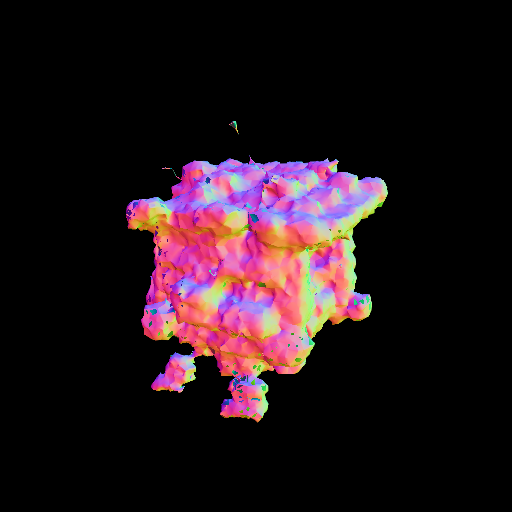
\includegraphics[width=\textwidth]{etc/a robot made out of plants/fantasia3d/fantasia_coarse_robot_5000_part2.png}
        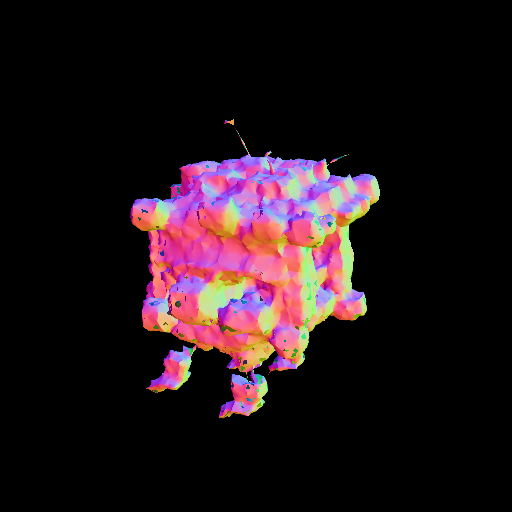
\includegraphics[width=\textwidth]{etc/a robot made out of plants/fantasia3d/fantasia_coarse_robot_10000_part2.png}
        \caption{}
    \end{subfigure}
    \begin{subfigure}[b]{0.20\textwidth}
        \centering
        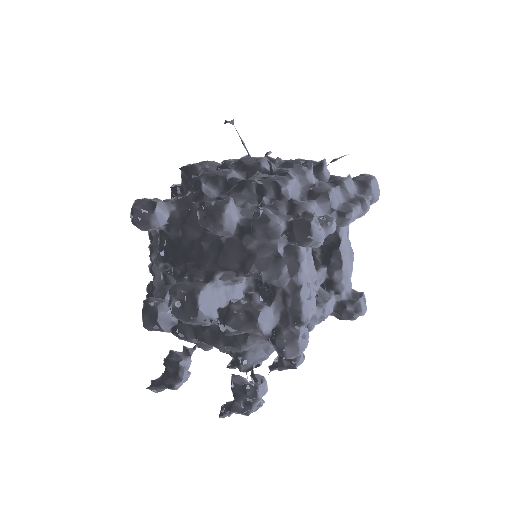
\includegraphics[width=\textwidth]{etc/a robot made out of plants/fantasia3d/fantasia_refine_robot_0_part1.png}
        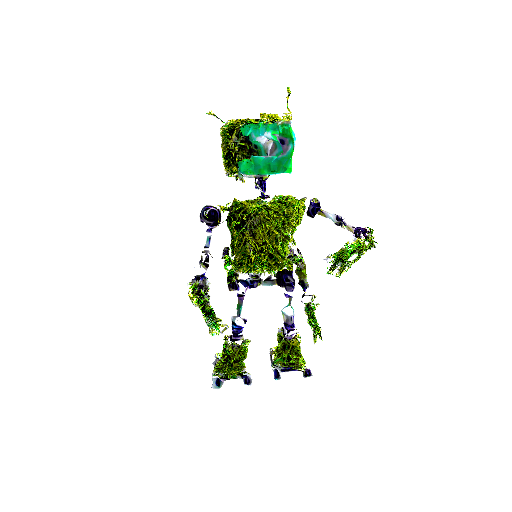
\includegraphics[width=\textwidth]{etc/a robot made out of plants/fantasia3d/fantasia_refine_robot_5000_part1.png}
        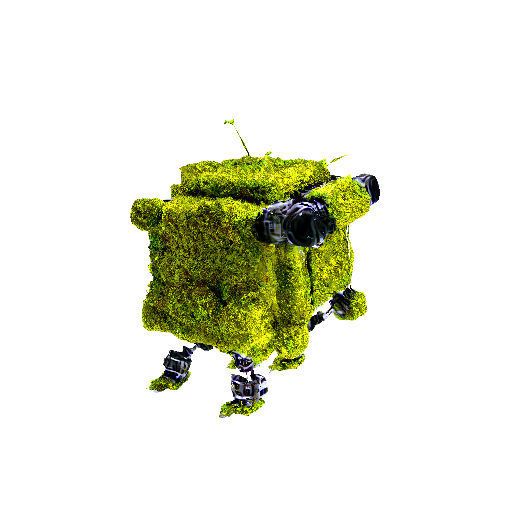
\includegraphics[width=\textwidth]{etc/a robot made out of plants/fantasia3d/fantasia_refine_robot_10000_part1.png}
        \caption{}
    \end{subfigure}
    % Subfigure 3
    \begin{subfigure}[b]{0.37\textwidth}
        \centering
        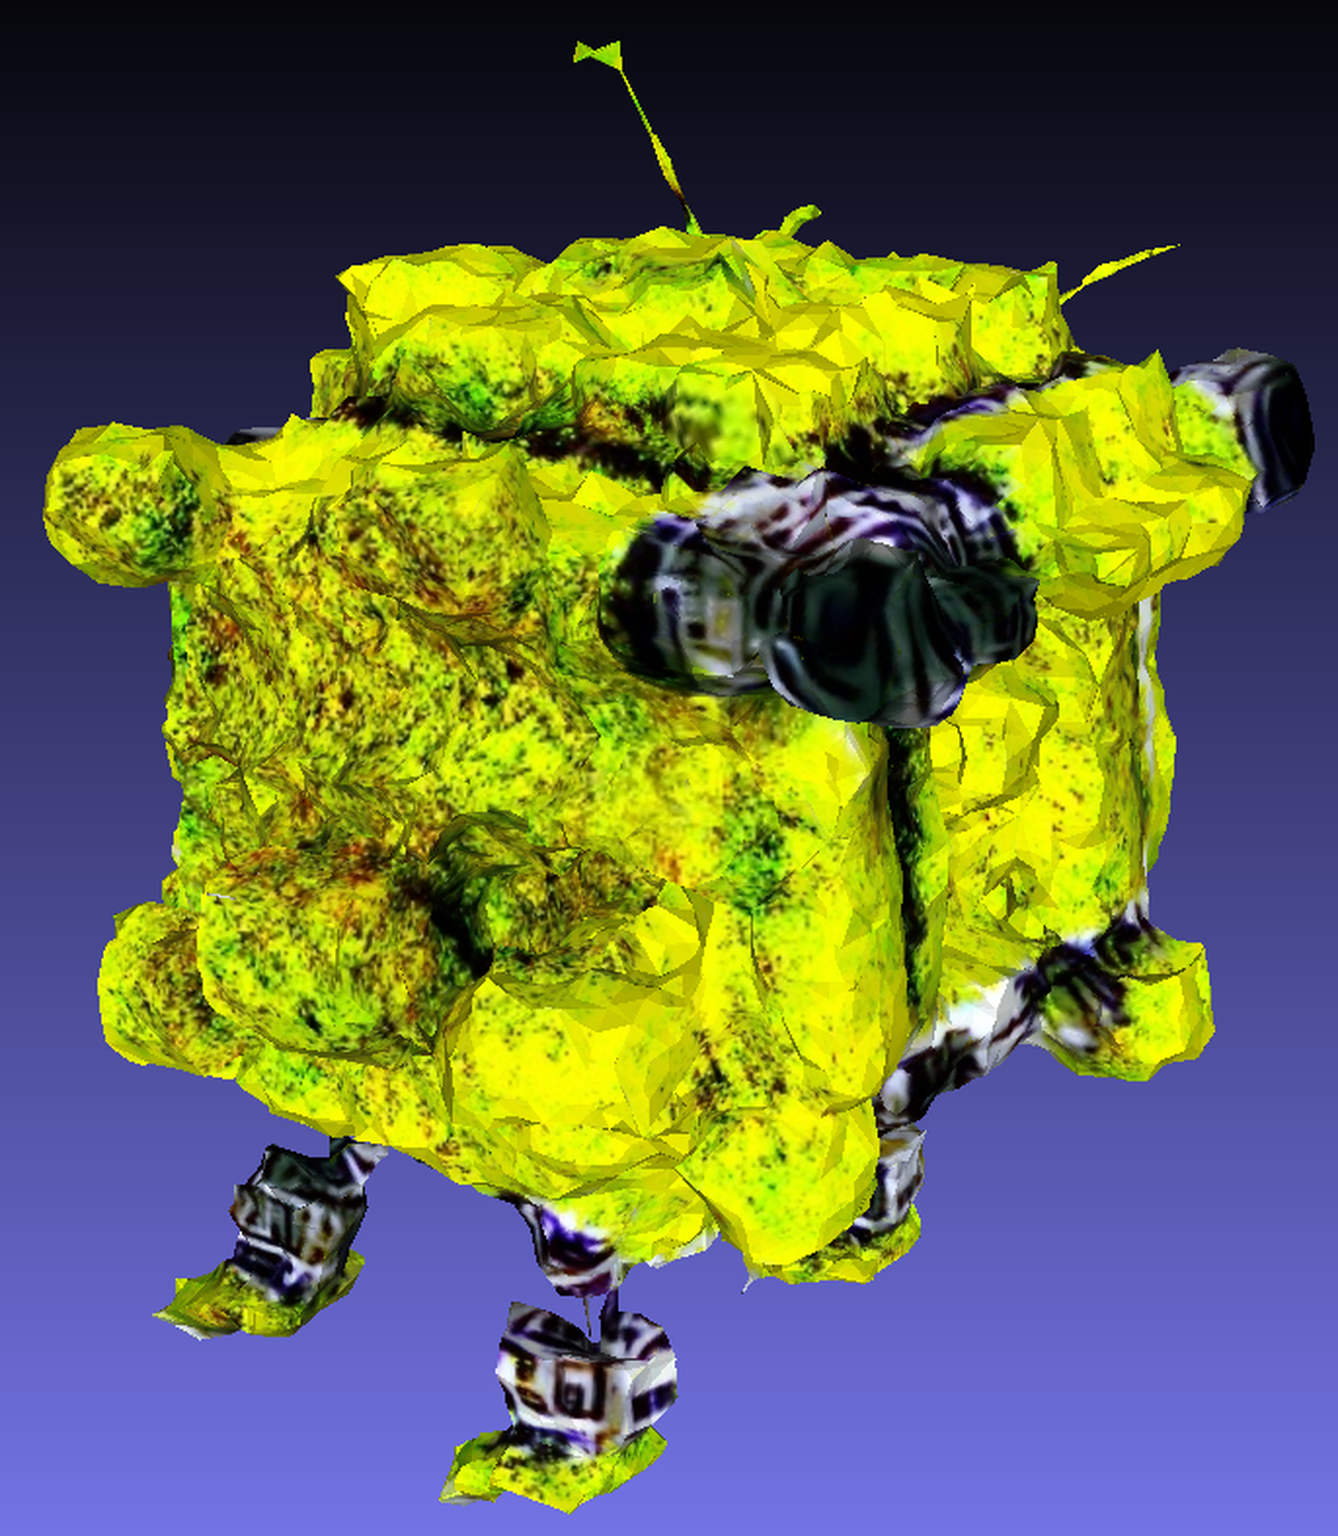
\includegraphics[width=\textwidth]{etc/a robot made out of plants/fantasia3d/fantasia_plantrobot_model_resized.png}
        \caption{}
    \end{subfigure}
    \caption{a: Fantasia3D starting with only a perfect square and refining this according to the prompt ``a robot made out of plants''. In b: only the appearance of the model gets refined. Image c shows the rendered model }~\label{fig:generationFantasia}
\end{figure}

Part (a) of Figure~\ref{fig:generationFantasia} illustrates the geometry stage of the method. Since only the prompt was used for initialization, Fantasia3D automatically selected a sphere as the base, influencing the overall quadratic shape of the final model. The figure reveals that the majority of the transformations occur between iterations 0 and 5000, where the sphere evolves, gaining corners and forming smaller blobs at the bottom, potentially interpreted as the robot's feet. However, at this geometry stage, it's challenging to discern the robot, especially as one made of plants. The changes from iteration 5000 to 10000 are more subtle, with slight smoothing in certain areas, such as the blob on the top left side of the robot or parts of the left foot, but these alterations are not significantly transformative.

Part (b) of the figure displays the appearance stage, where the model is textured. Starting with a greyscale base derived from the previous stage, the model gains color and texture as iterations progress. By iteration 5000, the texture, surprisingly resembling grass, enhances the model's detail and color, diminishing the prominence of the earlier clunky geometry. From iteration 5000 to 10000, this texture is further refined, introducing more detailed color variations and shadows, simulating light effects. Additionally, certain areas of the model exhibit metallic grey tones, particularly noticeable at the top right side and between the main body and the feet. 

However, some of these textural details are lost in the final mesh extraction, as seen in part (c). The model takes on a more yellowish hue, and the previously distinct lighting and shadows are reduced. Similar to the geometry stage, the final model does not clearly represent a robot made of plants; it more closely resembles a box with feet, akin to robots designed for food delivery. Throughout the training, Fantasia3D also generates various textures, including diffuse, roughness, metallic, and normals, as depicted in Figure~\ref{fig:generationFantasia}.

\begin{figure}[ht]
    \centering
      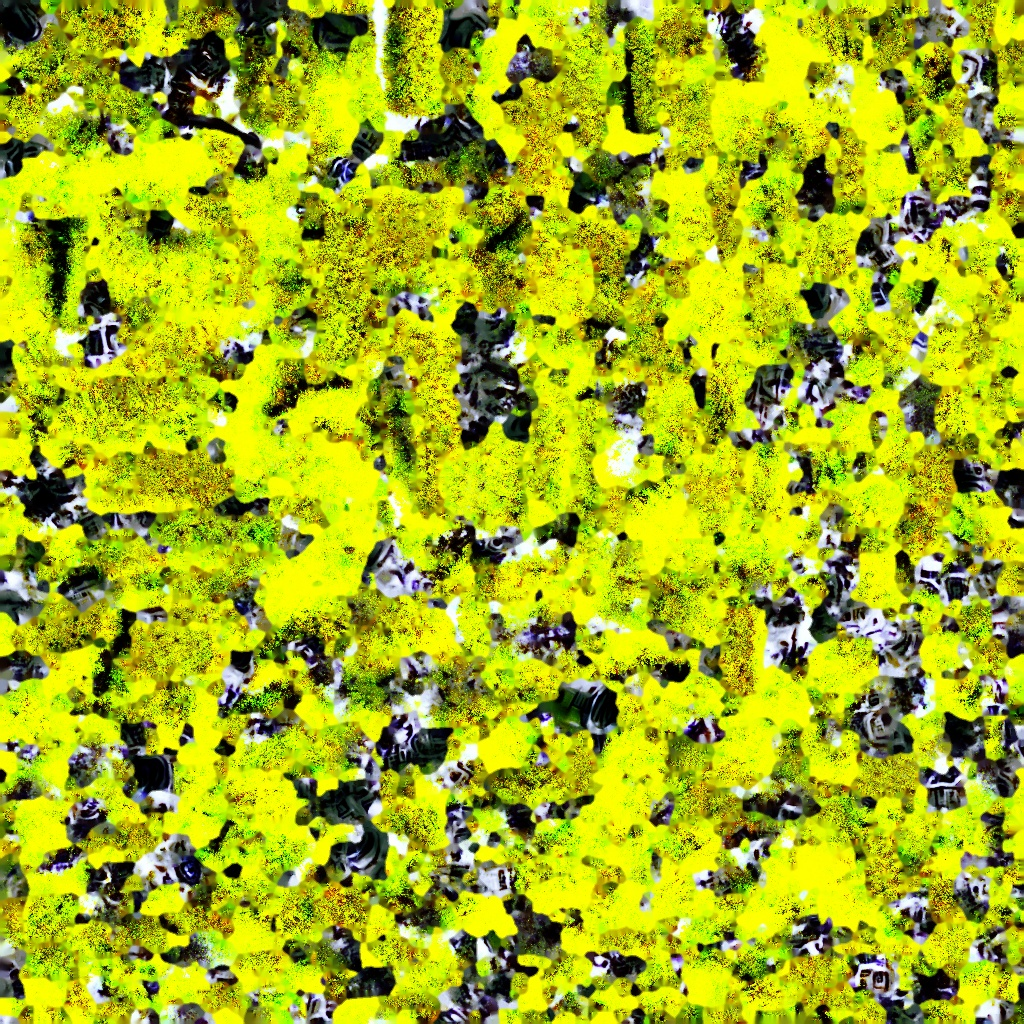
\includegraphics[width=.15\columnwidth]{etc/a robot made out of plants/fantasia3d/fantasia_refine_robot_kd}
      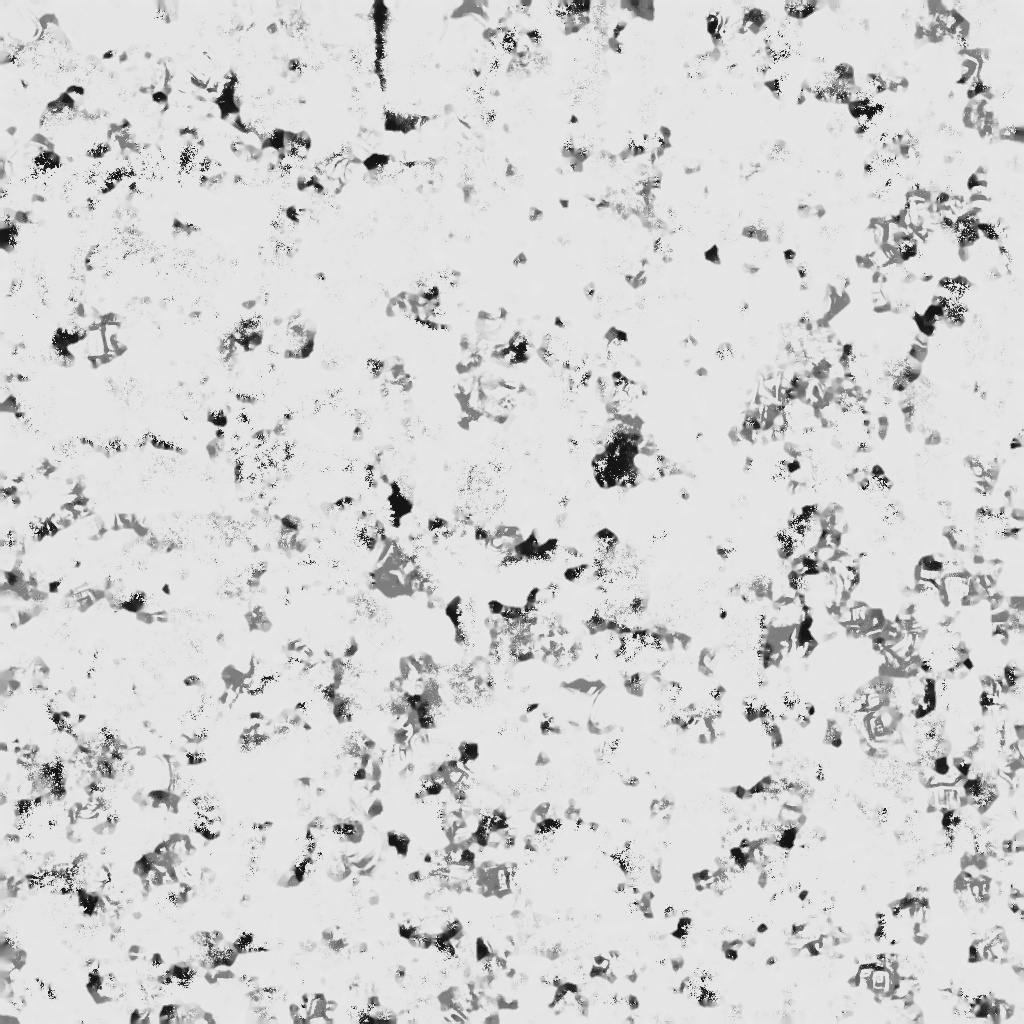
\includegraphics[width=.15\columnwidth]{etc/a robot made out of plants/fantasia3d/fantasia_refine_robot_roughness}
      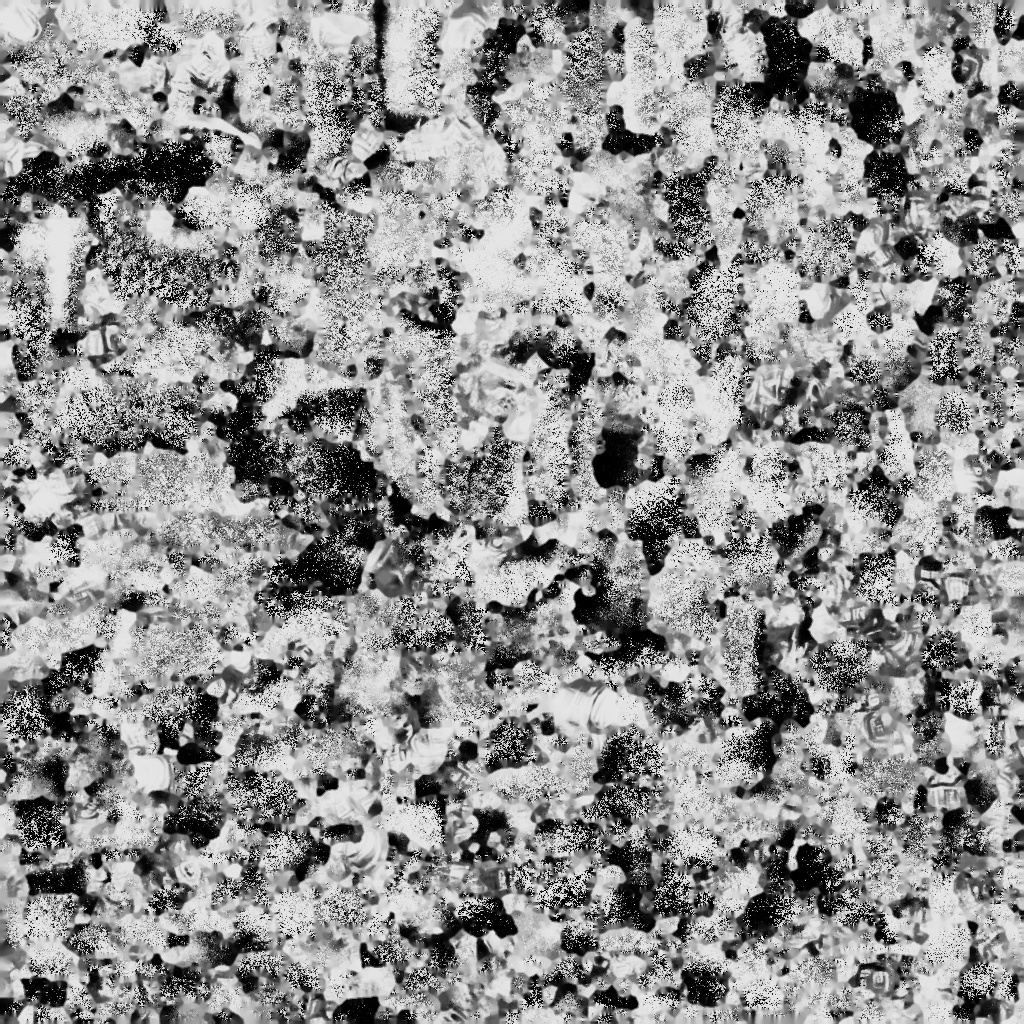
\includegraphics[width=.15\columnwidth]{etc/a robot made out of plants/fantasia3d/fantasia_refine_robot_metallic}
      
\includegraphics[width=.15\columnwidth]{etc/a robot made out of plants/fantasia3d/fantasia_refine_robot_normal}
      \caption{Generated textures from Fantasia3D\@; from left to right:  diffuse, roughness, metallic, and normal.}~\label{fig:texturesFantasia}
  \end{figure}


\textbf{Magic3D}~--~Magic3D employs a coarse-to-fine methodology, aiming to first construct a basic outline of the target object, which is then refined in subsequent stages to more accurately align with the text prompt. The mesh initialization is random, mirroring the approach used in DreamFusion.

\begin{figure}[ht]
    \centering
    % Subfigure for textual description
    \begin{subfigure}[b]{0.15\textwidth}
        \centering
        \fontsize{9pt}{7pt}\selectfont\text{Iteration = 200}\vspace{3cm}
        \fontsize{9pt}{7pt}\selectfont\text{It. 5000}\vspace{2.85cm}
        \fontsize{9pt}{7pt}\selectfont\text{It. 10000}\vspace{1.95cm}
    \end{subfigure}
    \begin{subfigure}[b]{0.2\textwidth}
        \centering
        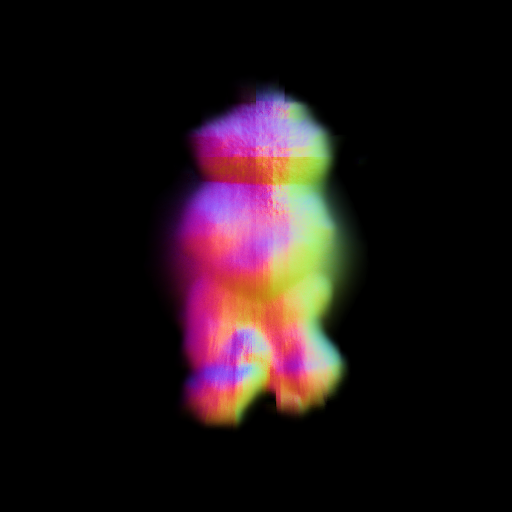
\includegraphics[width=\textwidth]{etc/a robot made out of plants/magic3d/magic3D_coarse_robot_0_part2.png}
        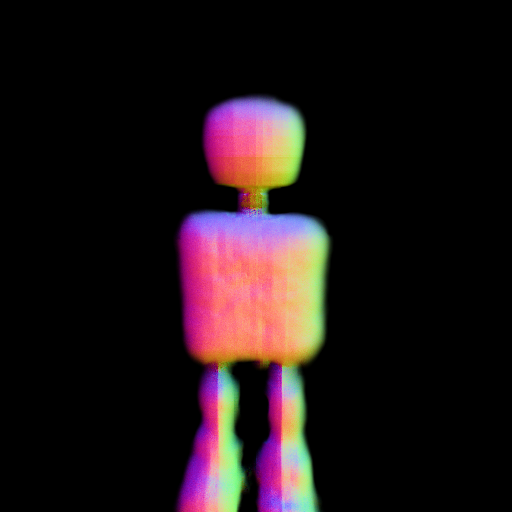
\includegraphics[width=\textwidth]{etc/a robot made out of plants/magic3d/magic3D_coarse_robot_5000_part2.png}
        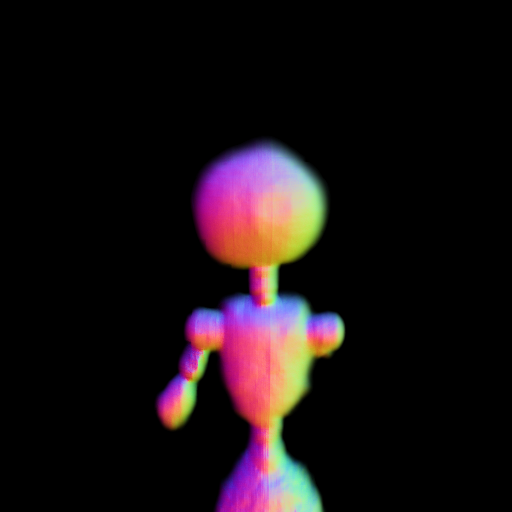
\includegraphics[width=\textwidth]{etc/a robot made out of plants/magic3d/magic3D_coarse_robot_10000_part2.png}
        \caption{}
    \end{subfigure}
    \begin{subfigure}[b]{0.2\textwidth}
        \centering
        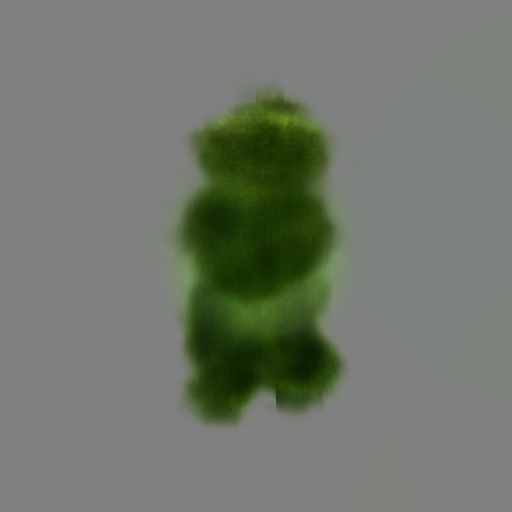
\includegraphics[width=\textwidth]{etc/a robot made out of plants/magic3d/magic3D_coarse_robot_0_part1.png}
        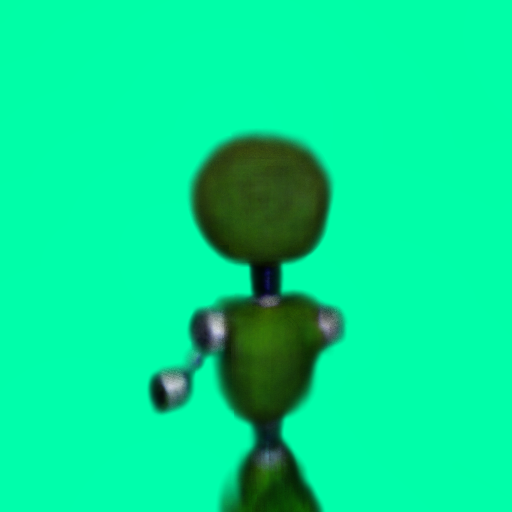
\includegraphics[width=\textwidth]{etc/a robot made out of plants/magic3d/magic3D_coarse_robot_5000_part1.png}
        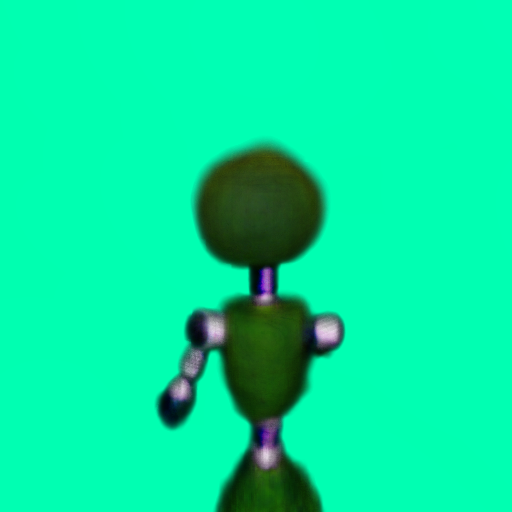
\includegraphics[width=\textwidth]{etc/a robot made out of plants/magic3d/magic3D_coarse_robot_10000_part1.png}
        \caption{}
    \end{subfigure}
    \begin{subfigure}[b]{0.2\textwidth}
        \centering
        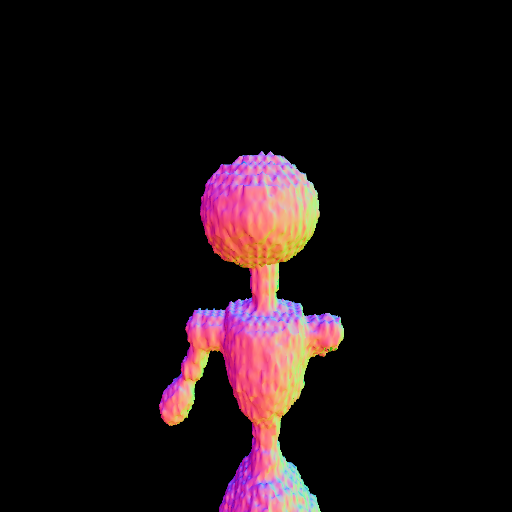
\includegraphics[width=\textwidth]{etc/a robot made out of plants/magic3d/magic3D_refine_robot_0_part2.png}
        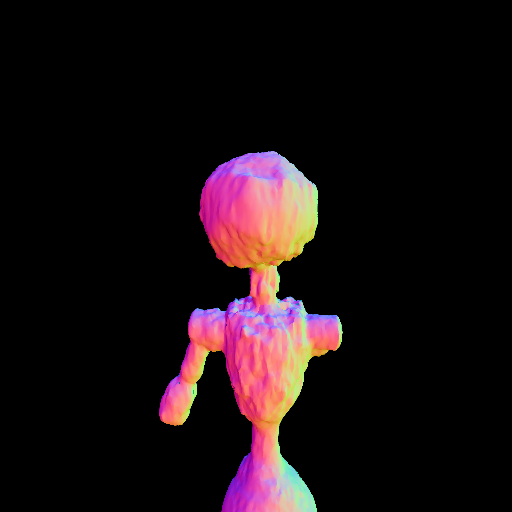
\includegraphics[width=\textwidth]{etc/a robot made out of plants/magic3d/magic3D_refine_robot_5000_part2.png}
        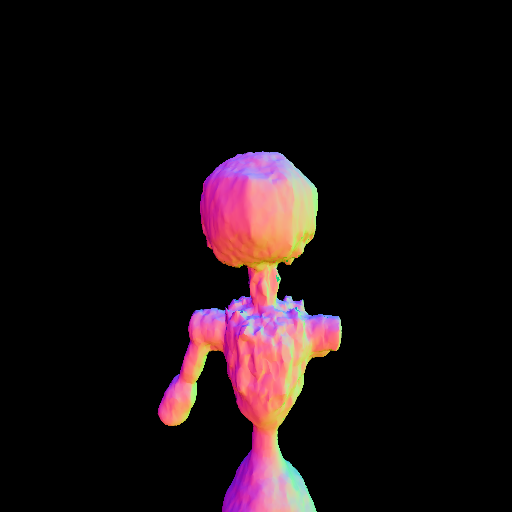
\includegraphics[width=\textwidth]{etc/a robot made out of plants/magic3d/magic3D_refine_robot_10000_part2.png}
        \caption{}
    \end{subfigure}
    \begin{subfigure}[b]{0.2\textwidth}
        \centering
        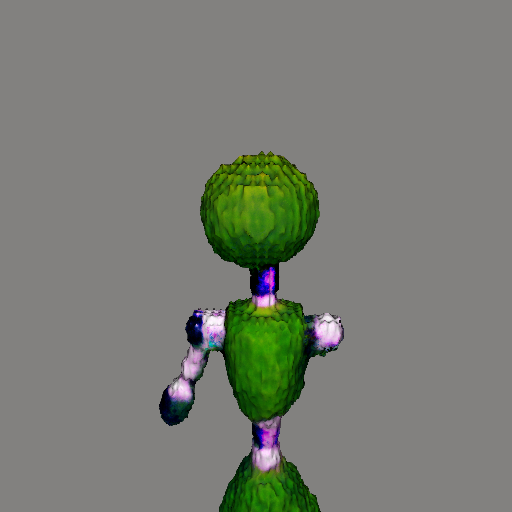
\includegraphics[width=\textwidth]{etc/a robot made out of plants/magic3d/magic3D_refine_robot_0_part1.png}
        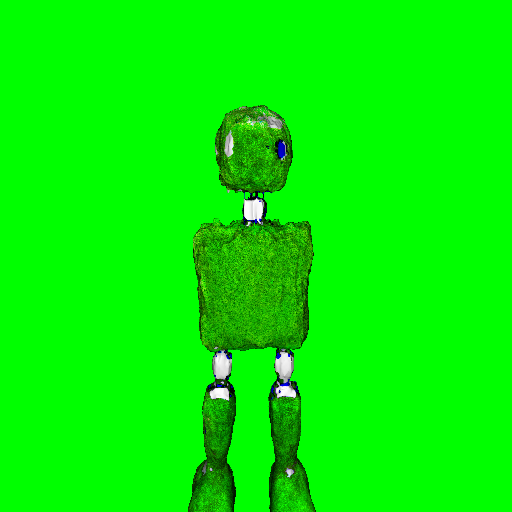
\includegraphics[width=\textwidth]{etc/a robot made out of plants/magic3d/magic3D_refine_robot_5000_part1.png}
        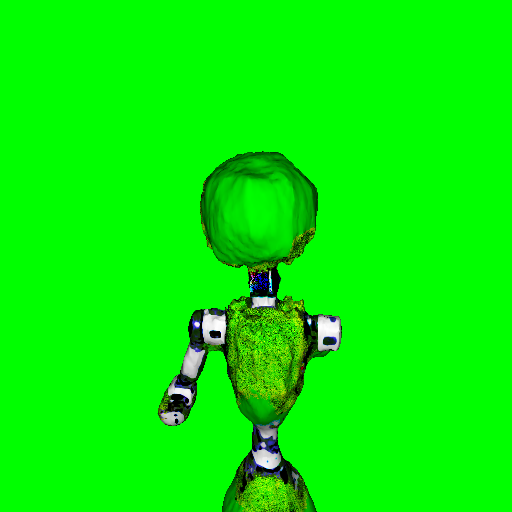
\includegraphics[width=\textwidth]{etc/a robot made out of plants/magic3d/magic3D_refine_robot_10000_part1.png}
        \caption{}
    \end{subfigure}
    \caption{Magic3D generation process from coarse (a, b) to fine (c, d)}~\label{fig:generationMagic3D}
\end{figure} 

The coarse stage can be seen in Figure~\ref{fig:generationMagic3D} parts (a) and (b). From a random start, a rough shape starts emerging by Iteration 200, accompanied by a plant-like green hue, setting the foundation for further refinement. By Iteration 5000, significant transformations have occurred from the initial stage: a distinct circular head, a neck, the upper body of the robot, and one arm have formed. The lower body, however, was omitted during training, forcing subsequent refinements on the upper half. At this point, the arm's color diverges from the green base, taking on a rough, grey-metallic appearance. Progressing to Iteration 10000, the neck and certain parts of the hip also adopt this metallic color. Despite these changes, the overall shape of the model sees only minor adjustments between Iteration 5000 and 10000, such as a thicker left arm and a more pronounced hip, but the right arm remains entirely absent. From the coarse stage alone, the model vaguely indicates a robotic form, with the plant aspect being derived primarily from the green coloring.

In the refinement stage, parts (c) and (d), the process starts from the model generated in the coarse stage. Initially, the mesh appears blocky but retains its original shape, with the neck, shoulder, and hip areas acquiring a purple hue between Iterations 0 and 200. By Iteration 5000, the model is smoother, with minor modifications to the head, losing some of its roundness. However, not much else changes in shape. The texture, though, sees significant refinement; the arms, hip, and neck gain more detail, resembling parts of an actual robot. The chest acquires grass-like detail and coloration. By Iteration 10000, some of these textural details diminish, as evidenced by the stomach area reverting to a plain green. However, the model gains light reflections, particularly noticeable on the shoulders. Despite these changes, the model's shape remains largely unchanged from Iteration 5000 to 10000, and the missing arm issue persists through the refinement stage.

The final mesh, as displayed in Figure~\ref{fig:texturesMagic3D}, is recognizable as a robot, and with close inspection, one might discern its grass-like chest, suggesting a plant-themed robot. For immediate and clear identification, the model would benefit from enhanced detail, particularly a more developed lower body extending beyond the hips. The left side of the figure displays the albedo generated during training.

\begin{figure}[ht]
    \centering
      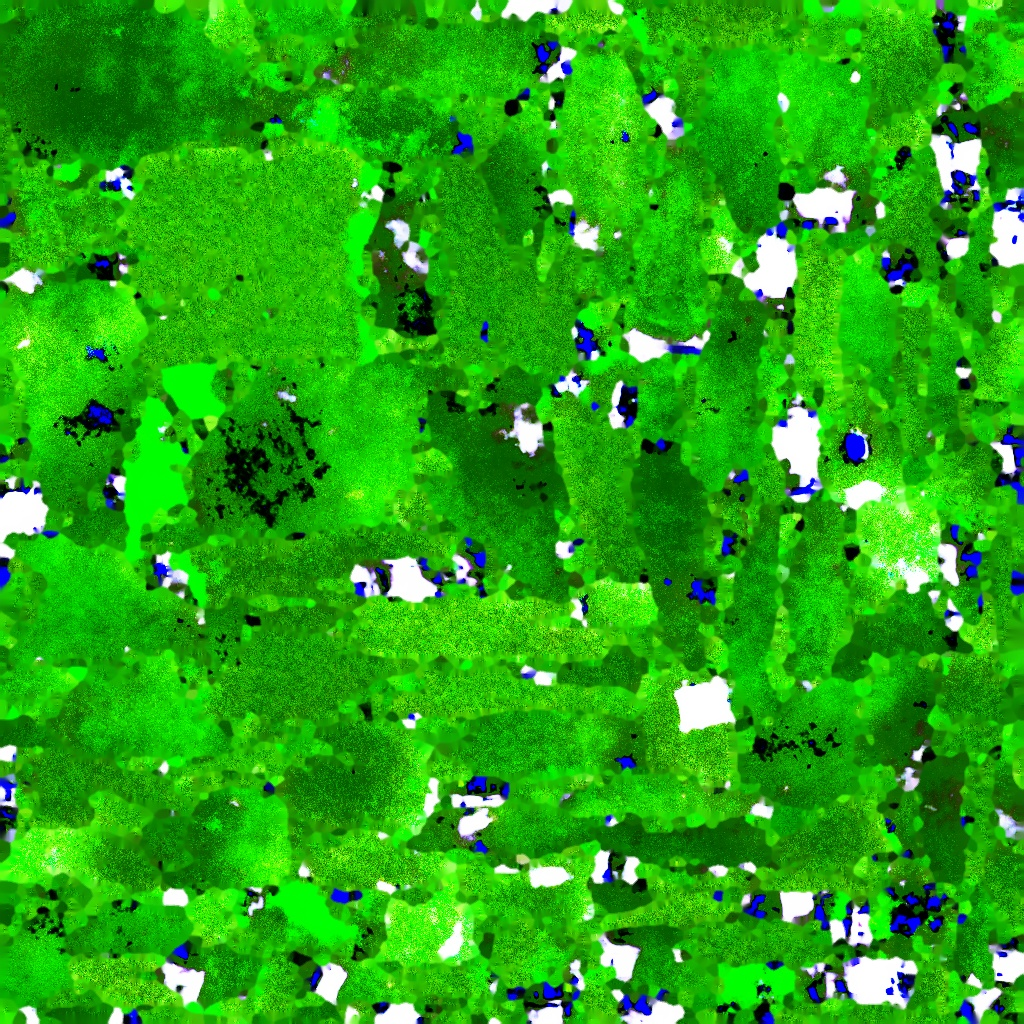
\includegraphics[width=.25\columnwidth]{etc/a robot made out of plants/magic3D/magic3D_refine_robot_texture}
      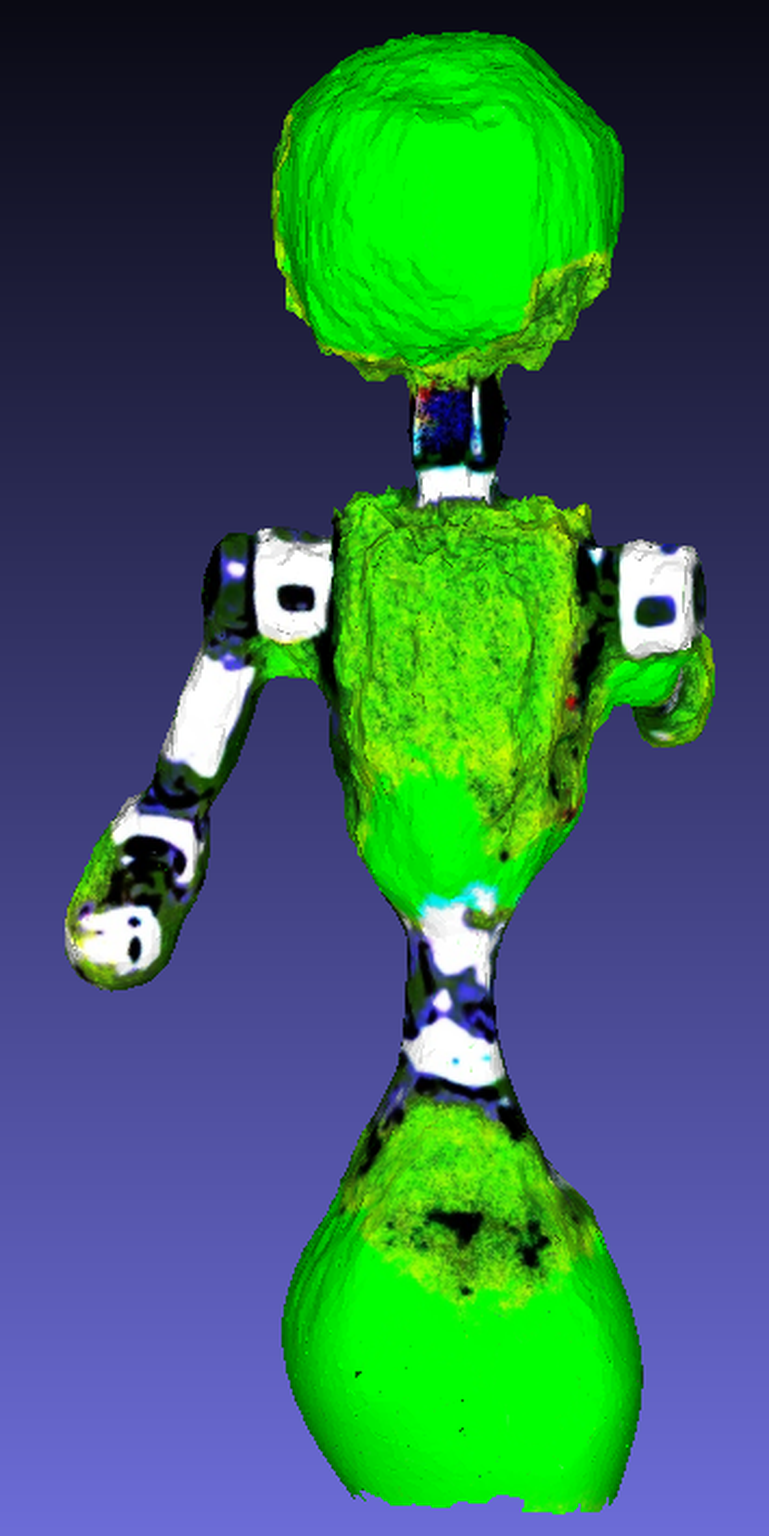
\includegraphics[width=.14\columnwidth]{etc/a robot made out of plants/magic3d/magic3d_plantRobot_model_resized.png}
      \caption{Magic3D also generates an albedo during training. The right side shows the extracted mesh.}~\label{fig:texturesMagic3D}
  \end{figure}



\textbf{magic123}~--~Test

\textbf{Wonder3D}~--~Test

\begin{figure}[ht]
    \centering
    \begin{subfigure}[b]{0.22\textwidth}
        \centering
        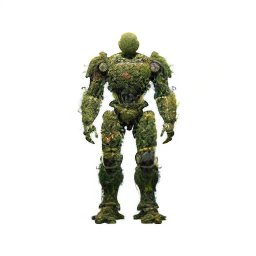
\includegraphics[width=\textwidth]{etc/a robot made out of plants/wonder3D/rgb_000_front.png}
        
\includegraphics[width=\textwidth]{etc/a robot made out of plants/wonder3D/normals_000_front.png}
        \caption{}
    \end{subfigure}
    \begin{subfigure}[b]{0.22\textwidth}
        \centering
        
\includegraphics[width=\textwidth]{etc/a robot made out of plants/wonder3D/rgb_000_front_right.png}
        
\includegraphics[width=\textwidth]{etc/a robot made out of plants/wonder3D/normals_000_front_right.png}
        \caption{}
    \end{subfigure}
    \begin{subfigure}[b]{0.22\textwidth}
        \centering
        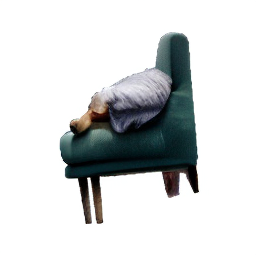
\includegraphics[width=\textwidth]{etc/a robot made out of plants/wonder3D/rgb_000_right.png}
        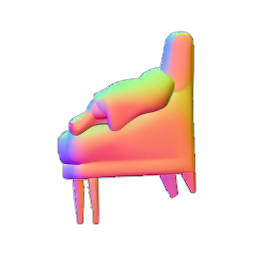
\includegraphics[width=\textwidth]{etc/a robot made out of plants/wonder3D/normals_000_right.png}
        \caption{}
    \end{subfigure}
    \hspace{5cm}
    \begin{subfigure}[b]{0.22\textwidth}
        \centering
        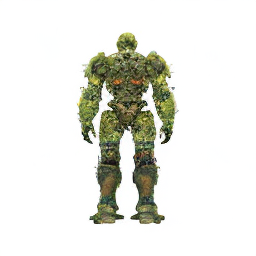
\includegraphics[width=\textwidth]{etc/a robot made out of plants/wonder3D/rgb_000_back.png}
        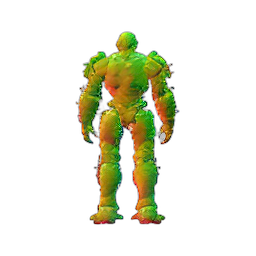
\includegraphics[width=\textwidth]{etc/a robot made out of plants/wonder3D/normals_000_back.png}
        \caption{}
    \end{subfigure}
    \begin{subfigure}[b]{0.22\textwidth}
        \centering
        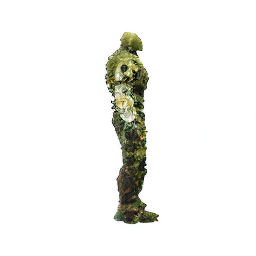
\includegraphics[width=\textwidth]{etc/a robot made out of plants/wonder3D/rgb_000_left.png}
        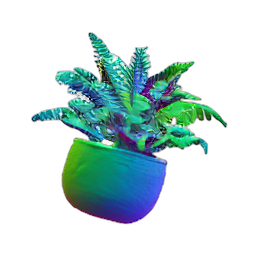
\includegraphics[width=\textwidth]{etc/a robot made out of plants/wonder3D/normals_000_left.png}
        \caption{}
    \end{subfigure}
    \begin{subfigure}[b]{0.22\textwidth}
        \centering
        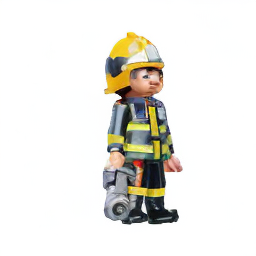
\includegraphics[width=\textwidth]{etc/a robot made out of plants/wonder3D/rgb_000_front_left.png}
        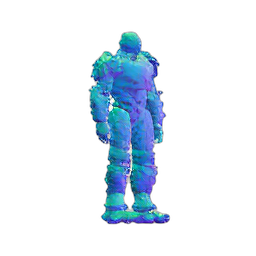
\includegraphics[width=\textwidth]{etc/a robot made out of plants/wonder3D/normals_000_front_left.png}
        \caption{}
    \end{subfigure}
    \caption{(a) front, (b) front right, (c) right, (d) back, (e) left, (f) front left}~\label{fig:generationWonder3D}
\end{figure}

\begin{figure}[ht]
    \centering
      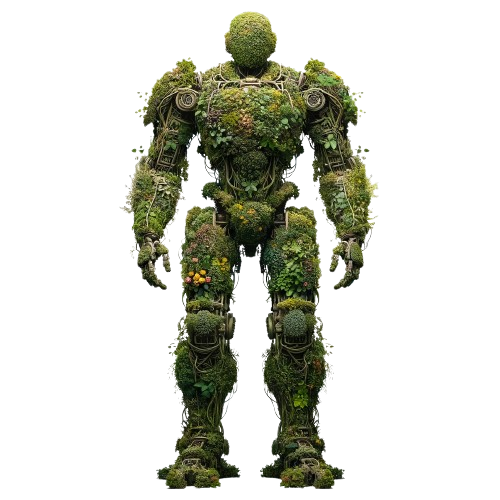
\includegraphics[width=.36\columnwidth]{etc/a robot made out of plants/wonder3d/plantRobot}
      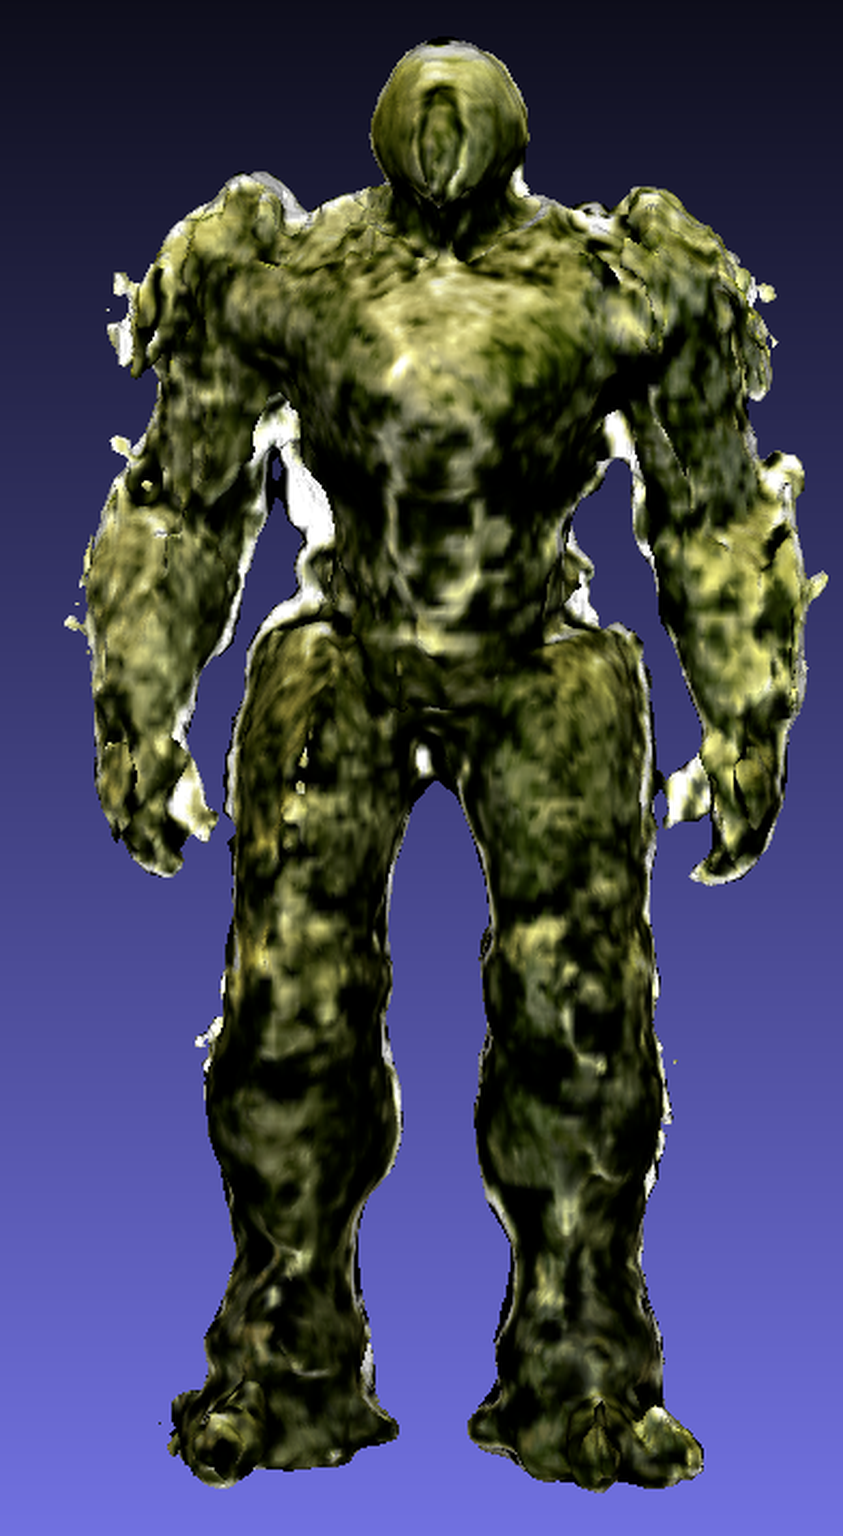
\includegraphics[width=.25\columnwidth]{etc/a robot made out of plants/wonder3d/wonder3d_plantrobot_model_resized}
      \caption{Generation of a 3D model (b) based on an imput image (a)}~\label{fig:inputWonder3d}
  \end{figure}
\section{Comparative Analysis}\label{comparativeAnalysis}

Conducting a comparative analysis of 3D models presents a challenging endeavor, as the parameters defining their success vary widely based on the intended application. For instance, low-resolution models suffice for real-time rendering in virtual reality or gaming contexts, whereas the film industry demands high-quality renderings. Similarly, in industrial applications, precision down to the millimeter is crucial, necessitating extremely detailed and accurate meshes. This analysis therefore approaches the assessment of generated models from multiple dimensions:

\begin{enumerate}
    \item \textbf{Prompt/Result Fidelity:} This dimension explores the alignment of each model with the original prompt and/or image. It questions whether the intended subject of the model is recognizable without prior knowledge of the input, thereby assessing the model's fidelity to the intended design.
    \item \textbf{Geometry:} Here, the focus is on the complexity and intricacy of each model. It evaluates whether the models exhibit detailed, fine structures or lean towards a more generalized, simplistic design. 
    \item \textbf{Texture Realism:} This aspect assesses the authenticity and quality of the textures applied to the models. It delves into questions of realism~-~how real do the textures appear?
\end{enumerate}

Following this subjective analysis, the study proceeds to evaluate technical aspects of each model, focusing on parameters such as rendering time, efficiency, and resource utilization. Each method is also subjected to targeted tests tailored to specific criteria. For instance, in scenarios where symmetry is critical, the models are evaluated for their ability to replicate symmetrical designs. Technical metrics for this analysis are derived from tensorboard data or outputs generated during the model training process. Detailed assessments and quantitative analyses~-~such as the evaluation of symmetry, and the detection of holes or anomalies in the models~-~are examined using Evaluate3D. This custom-developed tool integrates the trimesh Python library \citep{trimesh} to provide insights into the geometric properties of each 3D model.

\subsection{Subjective Evaluation}~\label{subjective}

In the preceding section, it was observed that the methods yielded diverse outcomes when tasked with a broad prompt, such as creating a `robot made of plants'. The text-to-3D methods faced challenges in initially generating an object, a stark contrast to the image-to-3D methods that benefited from having a reference image, offering some directional guidance and hence a slight advantage. To establish a more leveled playing field for the various methods, the next prompt chosen for testing was \textbf{``a high-quality rendering of a Playmobil firefighter''}. Playmobil figures are known for their uniform base structures, differing primarily in clothing or texture. This prompt was therefore selected to assess whether a method could accurately capture the fundamental structure dictated by the prompt. The outcomes of each method, applied to this specific prompt, are illustrated in Figure~\ref{fig:resultPlaymobil}. 

\begin{figure}[ht]
    \centering
    \small
    \begin{subfigure}[b]{0.18\textwidth}
        \centering
        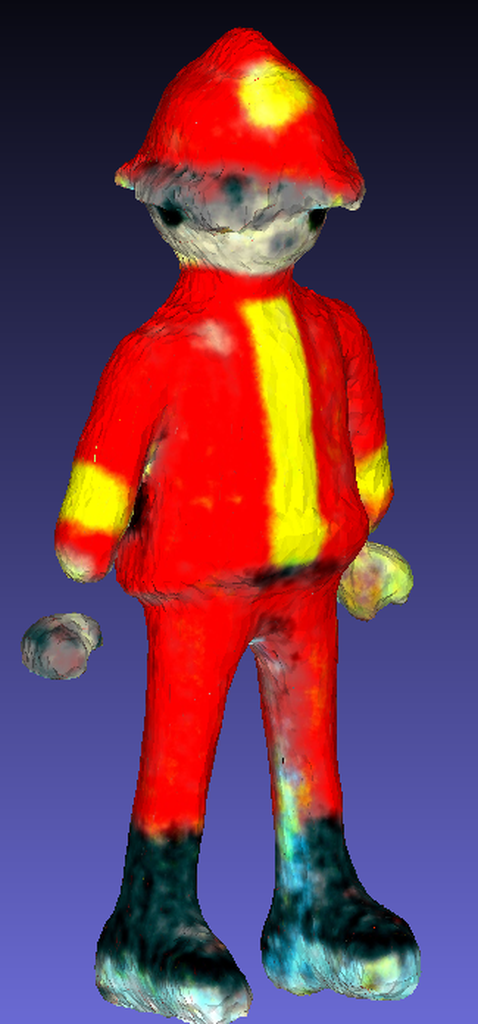
\includegraphics[width=\textwidth]{etc/a high quality rendering of a playmobil firefighter/dreamfusion/dreamfusion_playmobil_result_resize.png}
        \caption{DreamFusion}
    \end{subfigure}
    \begin{subfigure}[b]{0.179\textwidth}
        \centering
        
\includegraphics[width=\textwidth]{etc/a high quality rendering of a playmobil firefighter/magic3d/magic3d_playmobil_result_resize.png}
        \caption{Magic3D}
    \end{subfigure}
    \begin{subfigure}[b]{0.227\textwidth}
        \centering
        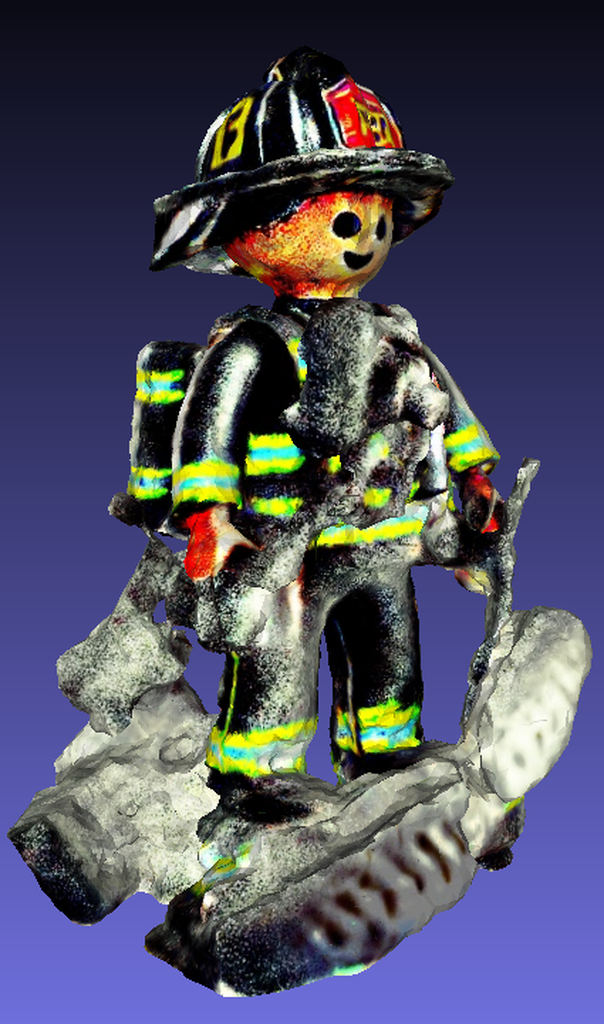
\includegraphics[width=\textwidth]{etc/a high quality rendering of a playmobil firefighter/fantasia3d_Magic3DInput/fantasia_playmobil_result_resize.png}
        \caption{Fantasta3D}
    \end{subfigure}
    \begin{subfigure}[b]{0.192\textwidth}
        \centering
        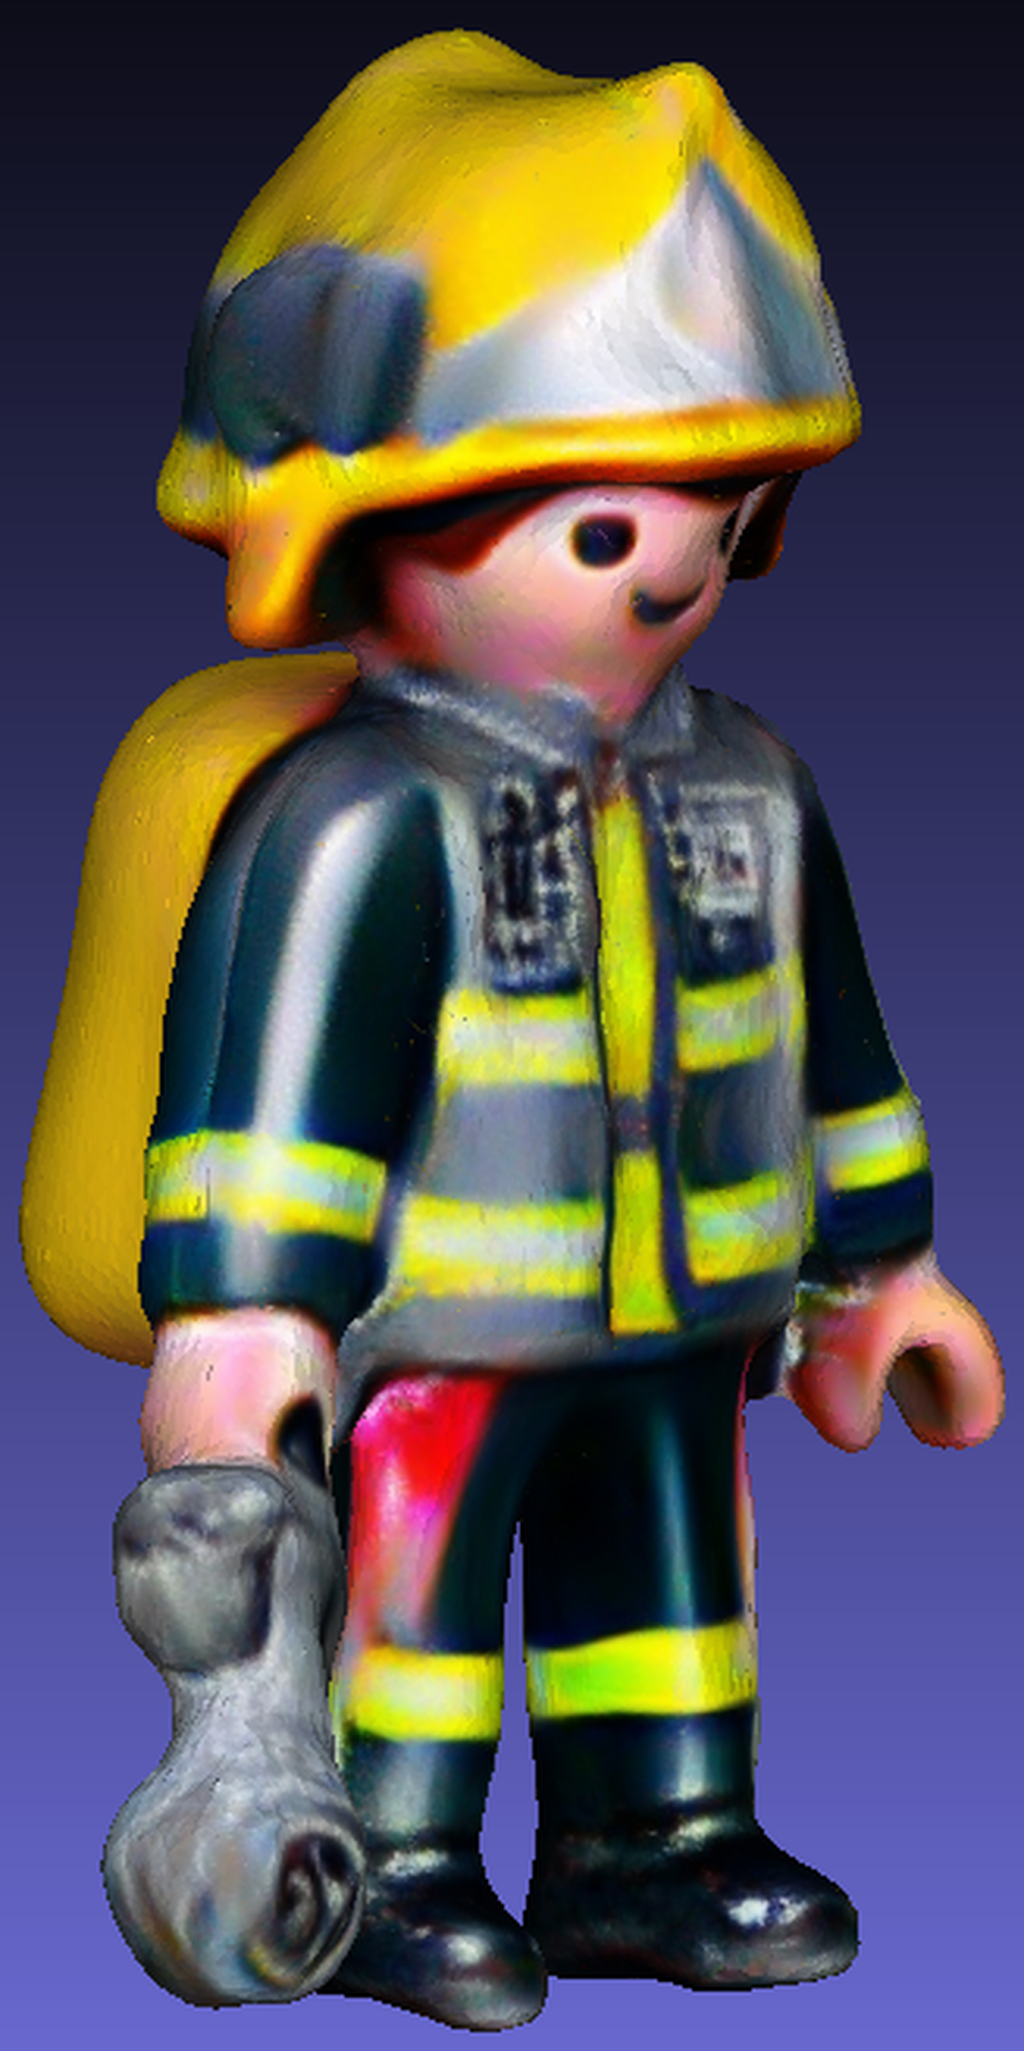
\includegraphics[width=\textwidth]{etc/a high quality rendering of a playmobil firefighter/magic123/magic123_playmobil_result_resize.png}
        \caption{Magic123}
    \end{subfigure}
    \begin{subfigure}[b]{0.181\textwidth}
        \centering
        \includegraphics[width=\textwidth]{etc/a high quality rendering of a playmobil firefighter/wonder3D/wonder3d_playmobil_result_resize.png}
        \caption{Wonder3D}
    \end{subfigure}
    \caption{Results obtained using the prompt ``a high-quality rendering of a Playmobil firefighter''.}~\label{fig:resultPlaymobil}
\end{figure}

\textbf{Prompt/Result Fidelity:} There is a clear split in the results when looking at fidelity to the prompt. DreamFusion and Magic123 tend to stick to the red clothing, while Fantasta3D, Magic123 and Wonder3D opt for a more realistic yellow and black firefighter uniform. Wonder3D and Magic123 adapt their results to the expected color scheme of the input image, given in Figure~\ref{fig:inputPlaymobil} part (a). Of particular interest is Fantasta3D's deviation from the red color scheme, although all models were refined with Stable Diffusion. This can be attributed to the physically based material model in the appearance stage, which has learned to associate firefighter clothing with yellow and black rather than red. Each model successfully reproduces identifiable Playmobil features such as helmets and uniforms, although the extent to which they reproduce the Playmobil style varies.

\textbf{Geometry:} The geometric shape of the models varies significantly. DreamFusion and Wonder3D present the most deviations from the expected Playmobil figure geometry. Both exhibit overly smooth shapes with ambiguous edges and floating elements, such as the hands in DreamFusion and around the right foot in Wonder3D, giving an unfinished appearance. In contrast, Fantasta3D achieves a promising silhouette but includes unintended additional objects, like a presumed fire extinguisher on the back and an ambiguous `thing' at the front, possibly an attempt at rendering a fire hose. Magic123, while delivering a solid representation, introduces a large bag on the figure's back, which, unlike the extraneous parts of Fantasta3D, integrates well with the overall model. A closer look of this bag is given in Figure~\ref{fig:inputPlaymobil} parts (b) and (c). Uniquely, Magic123 recreates the iconic Playmobil hand structure, complete with thumb, fingers, and the characteristic gap between them, capturing the essence of the figure's appendages. Magic3D impresses with a near-perfect rendering of the Playmobil figure, capturing the sharp transitions at the joints and maintaining smoothness elsewhere, except for a slight distortion around the feet. This result seems like one could bend and move it like it is possible with an original figure.

\textbf{Texture Realism:} In terms of texture, Magic3D again stands out with a level of realism that surpasses the others for the Playmobil prompt. It boasts clear demarcation between the colors, such as the black of the shoes against the red of the uniform, and the face retains the characteristic Playmobil look. The model's interaction with light, evidenced by chest reflections and inner leg shadows, adds to the plastic appearance. DreamFusion's model lacks such light interplay, resulting in a flat appearance, which is also caused due to the overall smoothened geometry. Fantasta3D, Magic123, and Wonder3D diverge from the red texture, opting for a black and yellow combination with realistic reflective stripes. Fantasta3D's texture is sound despite some geometric artifacts, with light reflection indicating a clear light source and giving the helmet a metallic sheen. Magic123 captures a plastic-like sheen, particularly on the arm's reflection, which underscores the roundness and smoothness of the figure. In contrast, Wonder3D's texture is not very detailed, blurs differences like the separation between jacket and shirt and does not render the character's face, similar to DreamFusion. The whole model looks strange, decayed and unfinished.

\begin{figure}[ht]
    \centering
    \small
    \begin{subfigure}[b]{0.25\textwidth}
        \centering
        \includegraphics[width=\textwidth]{etc/Images/playmobil.png}
        \caption{}
    \end{subfigure}
    \begin{subfigure}[b]{0.25\textwidth}
        \centering
        \includegraphics[width=\textwidth]{etc/a high quality rendering of a playmobil firefighter/magic123/magic123_playmobil_refine_back_10000_part1.png}
        \caption{}
    \end{subfigure}
    \begin{subfigure}[b]{0.25\textwidth}
        \centering
        \includegraphics[width=\textwidth]{etc/a high quality rendering of a playmobil firefighter/magic123/magic123_playmobil_coarse_right_10000_part1.png}
        \caption{}
    \end{subfigure}
    \caption{(a) displays the original image for the playmobil figure derived form Dall-E 3; (b and c) show the side and back view of Magic123, resectively}~\label{fig:inputPlaymobil}
\end{figure}

The next prompt used for the various methods was \textbf{``a rendering of a highly symmetrical loaf of bread''}. This prompt was selected to test the precision of each method in replicating detailed, specific requests while still producing coherent results. In this case, the model was tested for its symmetric result capability, which is discussed later in the technical section. The generated models are displayed in Figure~\ref{fig:resultBread}, which includes the original input image created by Dall-E 3 for reference.

Regarding \textbf{Prompt/Result Fidelity}, the outcomes varied. Magic123 and Magic3D successfully captured the essence of a bread, while Wonder3D produced an image that only vaguely suggested a loaf of bread. DreamFusion and Fantasia3D, however, were less successful; the former's result was indistinct, resembling a nondescript lump, while the latter's output more closely resembled a pineapple or an explosion when viewed without context.

\begin{figure}[ht]
    \centering
    \small
    \begin{subfigure}[b]{0.31\textwidth}
        \centering
        \includegraphics[width=\textwidth]{etc/a rendering of a highly symmetrical loaf of bread/dreamfusion/dreamfusion_bread_result.png}
        \caption{DreamFusion}
        \vspace{0.1cm}
    \end{subfigure}
    \begin{subfigure}[b]{0.31\textwidth}
        \centering
        \includegraphics[width=\textwidth]{etc/a rendering of a highly symmetrical loaf of bread/magic3d/magic3D_bread_result.png}
        \caption{Magic3D}
        \vspace{0.1cm}
    \end{subfigure}
    \begin{subfigure}[b]{0.2\textwidth}
        \centering
        \includegraphics[width=\textwidth]{etc/a rendering of a highly symmetrical loaf of bread/fantasia3d/fantasia_bread_result.png}
        \caption{Fantasta3D}
        \vspace{0.1cm}
    \end{subfigure}

    \begin{subfigure}[b]{0.269\textwidth}
        \centering
        \includegraphics[width=\textwidth]{etc/a rendering of a highly symmetrical loaf of bread/magic123/magic123_bread_result.png}
        \caption{Magic123}
        \vspace{0.1cm}
    \end{subfigure}
    \begin{subfigure}[b]{0.23\textwidth}
        \centering
        \includegraphics[width=\textwidth]{etc/a rendering of a highly symmetrical loaf of bread/wonder3D/wonder3d_bread_result.png}
        \caption{Wonder3D}
        \vspace{0.1cm}
    \end{subfigure}
    \begin{subfigure}[b]{0.23\textwidth}
        \centering
        \includegraphics[width=\textwidth]{etc/Images/bread.png}
        \caption{Original Image}
        \vspace{0.1cm}
    \end{subfigure}
    \caption{Results obtained using the prompt ``a rendering of a highly symmetrical loaf of bread''. Part (f) is the input image for Magic123 and Wonder3D, generated with Dall-E 3}~\label{fig:resultBread}
\end{figure}

In terms of \textbf{Geometry}, DreamFusion's model lacked meaningful structure, while Magic3D's bread model achieved good geometry, with a realistically carved top resembling fresh black bread. Fantasia3D, on the other hand, produced a model with a spikey appearance, potentially due to overfitting or difficulty in determining a starting point for the flat bottom of the bread. Magic123 excelled in replicating the geometry of the input image, closely matching the cuts and overall shape of the bread. Conversely, Wonder3D's model, like Fantasia3D's, had a roughly bread-like shape but suffered from spikey edges, possibly due to small adjustments during 3D mesh generation.

When considering \textbf{Texture Realism}, only the textures from Magic3D, Fantasia3D, and Magic123 seemed noteworthy. Magic3D's texture gave the impression of a burnt, dark loaf, with a realistic color gradient on the top. Although Fantasia3D's texture had a pleasing color combination, it resembled a cluster of breadsticks unless contextual information was provided. Magic123 accurately replicated the texture of the original image, demonstrating its proficiency in handling low-detail requirements.

To assess the methods' capability in reproducing smooth and reflective textures along with complex environmental details, the prompt \textbf{``a highly polished, seamless chrome sphere reflecting a complex cityscape in bright daylight''} was employed.





For a comprehensive evaluation of the methods' ability to render lifelike organic forms and textures, the prompt \textbf{``a high-quality rendering of a big dog sleeping on a chair''} was used. This particular prompt aims to test the realism in fur texture and the anatomical precision of the rendered dog.





To further explore each method's proficiency in rendering detailed natural elements and contrasting materials, the prompt \textbf{``a high-quality rendering of a fern in a wooden pot''} was introduced. This prompt serves to assess the handling of complex details in natural subjects, as well as the accuracy of color gradients and lighting in various levels of depth.


\begin{figure}[ht]
    \centering
    \small
    \begin{subfigure}[b]{0.24\textwidth}
        \centering
        \includegraphics[width=\textwidth]{etc/a high-quality rendering of a fern in a wooden pot/dreamfusion/dreamfusion_fern_result.png}
        \caption{DreamFusion}
        \vspace{0.1cm}
    \end{subfigure}
    \begin{subfigure}[b]{0.35\textwidth}
        \centering
        \includegraphics[width=\textwidth]{etc/a high-quality rendering of a fern in a wooden pot/magic3d/magic3d_fern_result.png}
        \caption{Magic3D}
        \vspace{0.1cm}
    \end{subfigure}
    \begin{subfigure}[b]{0.32\textwidth}
        \centering
        \includegraphics[width=\textwidth]{etc/a high-quality rendering of a fern in a wooden pot/fantasia3d/fantasia_fern_result.png}
        \caption{Fantasta3D}
        \vspace{0.1cm}
    \end{subfigure}

    \begin{subfigure}[b]{0.28\textwidth}
        \centering
        \includegraphics[width=\textwidth]{etc/a high-quality rendering of a fern in a wooden pot/magic123/magic123_fern_front_result.png}
        \caption{Magic123}
        \vspace{0.1cm}
    \end{subfigure}
    \begin{subfigure}[b]{0.27\textwidth}
        \centering
        \includegraphics[width=\textwidth]{etc/a high-quality rendering of a fern in a wooden pot/wonder3D/wonder3d_fern_result.png}
        \caption{Wonder3D}
        \vspace{0.1cm}
    \end{subfigure}
    \begin{subfigure}[b]{0.28\textwidth}
        \centering
        \includegraphics[width=\textwidth]{etc/Images/fern.png}
        \caption{Original Image}
        \vspace{0.1cm}
    \end{subfigure}
    \caption{Results obtained using the prompt ``a high-quality rendering of a fern in a wooden pot''.}~\label{fig:resultFern}
\end{figure}


\begin{figure}[ht]
    \centering
    \begin{subfigure}[b]{0.2\textwidth}
        \centering
        \includegraphics[width=\textwidth]{etc/a high-quality rendering of a fern in a wooden pot/magic123/magic123_fern_side_result.png}
        \caption{Magic123}
    \end{subfigure}
    \begin{subfigure}[b]{0.32\textwidth}
        \centering
        \includegraphics[width=\textwidth]{etc/a high-quality rendering of a fern in a wooden pot/wonder3D/rgb_000_right.png}
        \caption{Wonder3D}
    \end{subfigure}
    \caption{The side view of the fern showcasing the limitations of Magic123 in deriving the correct angles}\label{fig:fernSideview}
  \end{figure}



  \begin{figure}[ht]
    \centering
    \small
    \begin{subfigure}[b]{0.295\textwidth}
        \centering
        \includegraphics[width=\textwidth]{etc/a high-quality rendering of a big dog sleeping on a chair/dreamfusion/dreamfusion_dog_front_result.png}
        \caption{DreamFusion}
        \vspace{0.1cm}
    \end{subfigure}
    \begin{subfigure}[b]{0.32\textwidth}
        \centering
        \includegraphics[width=\textwidth]{etc/a high-quality rendering of a big dog sleeping on a chair/magic3d/magic3D_dog_front_result.png}
        \caption{Magic3D}
        \vspace{0.1cm}
    \end{subfigure}
    \begin{subfigure}[b]{0.33\textwidth}
        \centering
        \includegraphics[width=\textwidth]{etc/a high-quality rendering of a big dog sleeping on a chair/fantasia3d/fantasia_dog_front_result.png}
        \caption{Fantasta3D}
        \vspace{0.1cm}
    \end{subfigure}

    \begin{subfigure}[b]{0.267\textwidth}
        \centering
        \includegraphics[width=\textwidth]{etc/a high-quality rendering of a big dog sleeping on a chair/magic123/magic123_dog_front_result.png}
        \caption{Magic123}
        \vspace{0.1cm}
    \end{subfigure}
    \begin{subfigure}[b]{0.27\textwidth}
        \centering
        \includegraphics[width=\textwidth]{etc/a high-quality rendering of a big dog sleeping on a chair/wonder3D/wonder3D_dog_front_result.png}
        \caption{Wonder3D}
        \vspace{0.1cm}
    \end{subfigure}
    \begin{subfigure}[b]{0.28\textwidth}
        \centering
        \includegraphics[width=\textwidth]{etc/Images/dog.png}
        \caption{Original Image}
        \vspace{0.1cm}
    \end{subfigure}
    \caption{Results obtained using the prompt ``a high-quality rendering of a big dog sleeping on a chair''.}~\label{fig:resultDogFront}
\end{figure}


\begin{figure}[ht]
    \centering
    \small
    \begin{subfigure}[b]{0.291\textwidth}
        \centering
        \includegraphics[width=\textwidth]{etc/a high-quality rendering of a big dog sleeping on a chair/dreamfusion/dreamfusion_dog_back_result.png}
        \caption{DreamFusion}
        \vspace{0.1cm}
    \end{subfigure}
    \begin{subfigure}[b]{0.3\textwidth}
        \centering
        \includegraphics[width=\textwidth]{etc/a high-quality rendering of a big dog sleeping on a chair/magic3d/magic3D_dog_back_result.png}
        \caption{Magic3D}
        \vspace{0.1cm}
    \end{subfigure}
    \begin{subfigure}[b]{0.34\textwidth}
        \centering
        \includegraphics[width=\textwidth]{etc/a high-quality rendering of a big dog sleeping on a chair/fantasia3d/fantasia_dog_back_result.png}
        \caption{Fantasta3D}
        \vspace{0.1cm}
    \end{subfigure}

    \begin{subfigure}[b]{0.261\textwidth}
        \centering
        \includegraphics[width=\textwidth]{etc/a high-quality rendering of a big dog sleeping on a chair/magic123/magic123_dog_back_result.png}
        \caption{Magic123}
        \vspace{0.1cm}
    \end{subfigure}
    \begin{subfigure}[b]{0.27\textwidth}
        \centering
        \includegraphics[width=\textwidth]{etc/a high-quality rendering of a big dog sleeping on a chair/wonder3D/wonder3D_dog_back_result.png}
        \caption{Wonder3D}
        \vspace{0.1cm}
    \end{subfigure}
    \caption{Results obtained using the prompt ``a high-quality rendering of a big dog sleeping on a chair''.}~\label{fig:resultDogBack}
\end{figure}
\subsection{Technical Review}~\label{technical}

playmobil

The effectiveness of Evaluate3D is further enhanced by the integration of OpenAI's CLIP-score, a metric that quantifies the correspondence between an image and a given prompt \citep{radfordCLIP}. This is achieved by encoding both the prompt and the image into high-dimensional vectors within the same embedding space, and then determining the cosine similarity between these vectors. Cosine similarity is a measure of orientation rather than magnitude, with the cosine of the angle between two vectors indicating how closely the content of the image mirrors that of the text prompt. Despite its sophisticated design, this score is not without limitations and at times cannot rival the discerning capabilities of the human eye, occasionally leading to outcomes that may seem counterintuitive.

For convenience and to streamline the evaluation process, portions of the code using this metric have been integrated into Evaluate3D. This enables an immediate calculation of the CLIP-score post-rendering. Utilizing this feature, scores for the Playmobil figures have been computed and are presented in Table~\ref{table:scorePlaymobil}. In an intriguing turn, Magic123 ranks highest when assessed against the original prompt, followed by Fantasia3D, Wonder3D, DreamFusion, and finally, Magic3D. These findings are not entirely in concordance with the subjective analysis provided earlier. However, when the prompt is changed to ``a high-quality rendering of a red Playmobil firefighter'', there is a marked reversal in scores. This suggests that the CLIP-score may exhibit a bias towards the color black in the context of firefighter apparel, as opposed to the more toy-like red. The discrepancies highlighted by the CLIP-score accentuate the need for the development of new, more precise evaluation metrics tailored for assessing the output of 3D generative AI, as there currently exists no standard method that is universally recognized as reliable.

\begin{table}[h]
    \centering
    \small
    \begin{tabular}{lccccc}
    \toprule
    Prompt & DreamFusion & Magic3D & Fantasia3D & Magic123 & Wonder3D \\
    \midrule
    a Playmobil firefighter & 0.337 & 0.320 & 0.503 & 0.827 & 0.482 \\
    a red Playmobil firefighter & 0.501 & 0.604 & 0 & 0 & 0.216 \\
    \bottomrule
    \end{tabular}
    \caption{CLIP-scores for Playmobil firefighter models based on different prompts.}~\label{table:scorePlaymobil}
\end{table}


Bread

To quantitatively assess the symmetry of each model, the study employed Evaluate3D. This tool uses a function from trimesh to mirror a model along an axis and checks for corresponding vertices on the mirrored side. This process is repeated for all vertices, and a symmetry score is derived based on the number of matching pairs found. The findings of this assessment are detailed in Table~\ref{table:symmetrieBread}.

\begin{table}[ht]
    \centering
    \small
    \begin{tabular}{lccccc}
    \toprule
    {} & DreamFusion & Magic3D & Fantasia3D & Magic123 & Wonder3D \\
    \midrule
    Symmetrie Score & 0.337 & 0.320 & 0.503 & 0.827 & 0.482 \\
    \bottomrule
    \end{tabular}
    \caption{Symmetrie-scores for bread models demanding a symmetrical output.}~\label{table:symmetrieBread}
\end{table}



The blow table shows the rendering times required for each prmompt with each model. 

\begin{table}[ht]
    \centering
    \small 
    \begin{tabular}{lcccccccc}
    \toprule
    Prompt & DreamFusion & \multicolumn{2}{c}{Magic3D} & \multicolumn{2}{c}{Fantasia3D} & \multicolumn{2}{c}{Magic123} & Wonder3D \\
    \cmidrule(r){3-4} \cmidrule(lr){5-6} \cmidrule(l){7-8}
    & & \multicolumn{1}{c}{Coarse} & \multicolumn{1}{c}{Refine} & \multicolumn{1}{c}{Geom.} & \multicolumn{1}{c}{Appear.} & \multicolumn{1}{c}{C.} & \multicolumn{1}{c}{R.} &  \\
    \midrule
    Robot & 1:24 & 1:23 & 1:20 & 1:15 & 1:18 & 1:46 & 1:47 & 0:15 \\
    Playmobil & 1:17 & 1:17 & 1:18 & 1:14 & 1:17 & 1:46 & 1:46 & 0:15 \\
    Fern & 1:25 & 1:24 & 1:19 & 1:17 & 1:20 & 1:52 & 1:48 & 0:15 \\
    Bread & 1:25 & 1:21 & 1:21 & 1:17 & 1:20 & 1:54 & 1:52 & 0:15 \\
    \bottomrule
    \end{tabular}
    \caption{Comparison of Generation Times for Different Prompts Across Methods (Hours:Minutes). Legend: C = Coarse, R = Refine, Geom = Geometry, Appear = Appearance.}~\label{table:generation_times_complex}
\end{table}

 
    
    
    